\documentclass[10pt,letterpaper,twoside]{article}
\usepackage[latin1]{inputenc}
\usepackage[pdftex]{graphicx}     % Add some packages for figures. Read epslatex.pdf on ctan.tug.org
\usepackage{geometry}
\usepackage{fancyhdr}
\usepackage{amsmath}
\usepackage{amsfonts}
\usepackage{bm}
\usepackage{outlines}
\usepackage{calligra}
%\usepackage{pxfonts}
%\usepackage[T1]{fontenc}{pxfonts}
%\usepackage{newpxtext,newpxmath}
\usepackage{mathrsfs}
\usepackage{units}
\usepackage{amssymb}
\usepackage{titlesec}
\usepackage[section]{placeins}
\usepackage{color}
\usepackage[labelfont={normal,bf},font=normal]{caption}
\usepackage[activate={true,nocompatibility},final,tracking=true,kerning=true,spacing=true,factor=1200,stretch=20,shrink=20]{microtype}
\usepackage[colorlinks=true,
			linkcolor=webgreen, %defined below
			filecolor=webbrown, %defined below
			citecolor=webgreen, %defined below
			%------------- Doc Info ---------------------------------
			pdftitle={Finding the electric field directly from a charge distribution: Coulomb's law and Gauss's law},
			pdfauthor={J. L. Lanfranchi},
			pdfsubject={},
			pdfkeywords={},
			%------------ Doc View ----------------------------------
			bookmarksopen=true,
			pdfpagemode=UseOutlines]{hyperref}
\definecolor{mygreen}{rgb}{0,0.6,0}
\definecolor{mygray}{rgb}{0.5,0.5,0.5}
\definecolor{mymauve}{rgb}{0.58,0,0.82}
\definecolor{webgreen}{rgb}{0.0,0,0.8}
\definecolor{webgreen}{rgb}{0.0,0,0.8}
\definecolor{webbrown}{rgb}{0,0,0.8}
\usepackage{calligra}
\DeclareMathAlphabet{\mathcalligra}{T1}{calligra}{m}{n}
\DeclareFontShape{T1}{calligra}{m}{n}{<->s*[2.2]callig15}{}
\newcommand{\scripty}[1]{\ensuremath{\mathcalligra{#1}}}

\setlength{\floatsep}{0.01in}
\setlength{\textfloatsep}{0.01in}
\setlength{\topmargin}{0.01in}
\setlength{\topskip}{0.01in}
\setlength{\textheight}{0.1in}
\setlength{\intextsep}{3pt}

\newcommand{\sectionlinetwo}[2]{%
  \nointerlineskip \vspace{.5\baselineskip}\hspace{\fill}
  {\resizebox{0.5\linewidth}{1.2ex}
    {\pgfornament[color = #1]{#2}
    }}%
    \hspace{\fill}
    \par\nointerlineskip \vspace{.5\baselineskip}
  }

\author{J. L. Lanfranchi}
%\email{jll1062@phys.psu.edu}
\title{Finding the electric field directly from a charge distribution:\\
Coulomb's law and Gauss's law}
\geometry{top=0.70in,left=0.70in,right=0.70in,bottom=0.70in}
\begin{document} 
\twocolumn
\maketitle
\section{Background}
There are two equations (or rather two forms of the same equation) that we can use to find $\bm E$ directly from a charge distribution: Coulomb's law and Gauss's law.
Note first that $\bm E$ is a vector whose magnitude and direction change by coordinate; i.e., it's a vector function of three dimensions: $\bm E(\bm r)$, or $\bm E(x,y,z)$, or $\bm E(r,\theta,z)$, or $\bm E(r,\theta,\phi)$, depending upon how you want to write the coordinate.

With certain symmetries in the problem, you can work out the integral that Coulomb's law leads to. Other situations lend themselves to use of Gauss's law.
A third way, which I'm not addressing here, is to first find the electric potential and then use $\bm E=-\bm\nabla V$ to find the electric field.
Something for another write-up, but note that the math I describe here generalizes to that method as well.

\section{Coulomb's Law}
First, starting with Coulomb's law for a point charge, we see that the point charge causes an electric field $\bm E_i$ at some point in space $\bm r$ according to the equation
\begin{equation}\bm{E_i(r)} = k\frac{Q}{r_i^2}\bm{\hat r}_i \label{eqn:coulomb0}\end{equation}
where $\bm{r}_i$ is the vector pointing \textit{from} the charge \textit{to} the point in space at which we're finding the E-field (see Fig.~\ref{fig:coord_coulomb}).

%-------------------------------------------------------------------------------
\begin{figure}[htb]
  \centering
  \vspace{5pt}
  \hrule%{2in}{0.5pt}
  \vspace{10pt}
  %\begin{minipage}[l]{1.0\columnwidth}
	\centering
	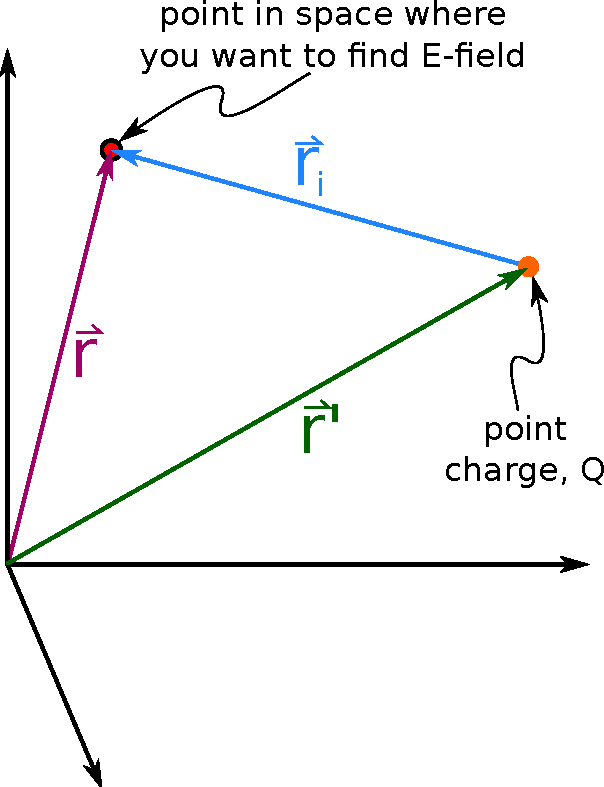
\includegraphics[keepaspectratio=true,width=1.50in]{./coordinate_system_single_charge.pdf}
    \caption{Geometry for analyzing the E-field due to a point charge.
			 Note that only the vector $\bm r_i$ and its associated unit vector, $\bm{\hat r}_i$, enter into the RHS of Eqn.~\ref{eqn:coulomb0}.
			 That's where the \textit{physics} is in this picture!}
    \label{fig:coord_coulomb}
  %\end{minipage}
  \hrule%{2in}{0.5pt}
\vspace{5pt}
\end{figure}
%\FloatBarrier
%-------------------------------------------------------------------------------

But we have a whole distribution of charge, so instead of just a \textit{single} charge $Q$, we need to add up (superposition's our friend!) the contributions to the electric field from every little bit of charge, $\text{d}Q$, in the overall charge distribution.
We could beat around the bush here, but there's a very nice mathematical tool for adding up lots of little things (the integral), so we're going to use it, without fear and without hate, where we can:
\begin{equation}
\bm{E(r)} = \int\limits_{\substack{\text{everywhere}\\\text{there's\,charge}}} k\frac{\bm{\hat r}_i}{{r_i}^2}\;\mathrm{d}Q\label{eqn:coulomb1} \\
\end{equation}
(Refer to Fig.~\ref{fig:coord_coulomb_distr} for the geometry involved in this equation.)
Unfortunately this can be a prohibitively tricky integral to work out since each different bit of charge $\text d Q$ has a different $\bm r_i$ and so a different (up to) 3-component vector $\bm{\hat r}_i$ that must be summed over.

%-------------------------------------------------------------------------------
\begin{figure}[htb]
  \centering
  \vspace{5pt}
  \hrule%{2in}{0.5pt}
  \vspace{10pt}
  %\begin{minipage}[l]{1.0\columnwidth}
	\centering
	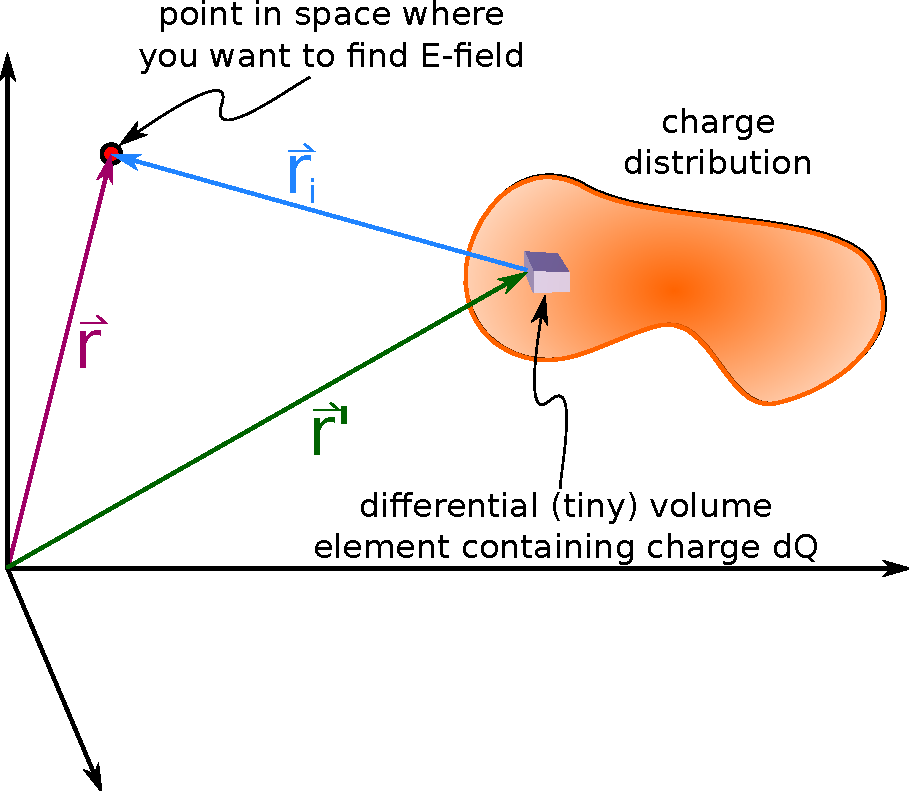
\includegraphics[keepaspectratio=true,width=2.50in]{./coordinate_system.pdf}
    \caption{Geometry for analyzing the E-field due to a charge distribution.
	The \textit{physics} for each little bit of the sum is due to the differential charge element $\text d Q$ and the vector $\bm r_i$ pointing from $\text d Q$ to the point $\bm r$ where you're trying to find the E-field; hence, these are what show up \textit{explicitly} in the integrand of Eqn.~\ref{eqn:coulomb1}.
	The integral is taken over all of the charge distribution, so the coordinates that make up $\bm r'$ show up when we break $\text d Q$ down and we get a purely geometrical part ($\text d x'\,\text d y'$ in plane-Cartesian coordinates).
	So $\bm r'$ is the variable of integration (and so also shows up in the limits of integration), as can be seen in Eqn.~\ref{eqn:coulomb2}.}
    \label{fig:coord_coulomb_distr}
  %\end{minipage}
  \hrule%{2in}{0.5pt}
\vspace{10pt}
\end{figure}
%\FloatBarrier
%-------------------------------------------------------------------------------

I'm about to delve deeper into the \textit{process} and \textit{math} involved in calculating the E-field from Coulomb's law.
But don't tune out!
It's similar to computing the electrostatic potential from a charge distribution, and the ideas behind working these integrals also generalize to the surface and volume integrals you'll find in Gauss's law.

It's your first job to think about what a small bit of charge looks like for the distribution you're given and in the coordinate system you've chosen.
If you're given a charge density (linear, surface, or volume), then you can write $\text d Q = (\text{charge\,dens}) \cdot \text d V$ where $\text d V$ is the differential ``volume'' element appropriate to the distribution's dimensionality and your coordinate system.
Remember that $\text d Q$ has units of charge (e.g., C in SI), so if you know the surface charge density $\eta$, which has units C/m$^2$, you know that your differential ``volume'' element $\text d V$ must consist of two lengths to make the overall units end up as C; for this example, and using Cartesian coordinates, you should get $\text d Q = \eta \, \text d x'\,\text d y'$.

Note that $\eta$ may change with location in space, and so be dependent upon some components (or all) of $\bm r'$.
Note also that I use primes (') to indicate the coordinate that you're \textit{summing over}, $\bm{r'}$, which has Cartesian coordinates $(x',y')$ in 2D; refer again to Fig.~\ref{fig:coord_coulomb_distr}.

Summarizing this discussion of Coulomb's law for a surface charge density in Cartesian coordinates is the equation
\begin{equation}
  \bm E(\bm r) = \int\limits_{y'=?}^{?}\int\limits_{x'=?}^{?} k\frac{\eta(x',y')\,\bm{\hat r}_i}{{r_i}^2}\;\mathrm{d}x' \, \text d y'.\label{eqn:coulomb2}
\end{equation}

If you're using polar coordinates, e.g. plane polar coordinates $(r',\theta')$, remember that \textit{an angle has no units} (sadly for radians, they just don't count!), so $\text d \theta'$ has no units and hence the differential ``volume'' \textbf{cannot just involve} $\text d r'$ \textbf{and}  $\text d \theta'$.
Of course all confusion is avoided when you draw a picture of your differential ``volume'' element and you identify what the lengths of each side are, based upon that picture; see Fig.~\ref{fig:plane_polar_dr}.

%-------------------------------------------------------------------------------
\begin{figure}[htb]
  \centering
  \vspace{5pt}
  \hrule%{2in}{0.5pt}
  \vspace{10pt}
  %\begin{minipage}[l]{1.0\columnwidth}
	\centering
	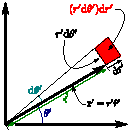
\includegraphics[keepaspectratio=true,width=2.1in]{./plane_polar_dr.pdf}
    \caption{Geometry for finding a differential ``volume'' element in 2D using plane-polar coordinates.
	         Tweak the vector's coordinate $\theta'$ (angle) a little (by an a\ointmount $\text d \theta'$), and the vector rotates a bit, tracing out an arc of length $r'\,\text d\theta'$.
	         Tweak the vector's coordinate $r'$ (magnitude) a little (by an amount $\text d r'$), and the vector gets longer, tracing out the length $\text d r'$.
			 Multiply these, and the differential ``volume'' element has an area $\left( r'\,\text d \theta' \right)\text d r'$.}
    \label{fig:plane_polar_dr}
  %\end{minipage}
  \hrule%{2in}{0.5pt}
\vspace{5pt}
\end{figure}
%\FloatBarrier
%-------------------------------------------------------------------------------

\section{Gauss's law}
If a charge $Q$ is present somewhere in space, it ``produces'' an E-field.
Surrounding this charge with a closed surface, and using Coulomb's Law along with the divergence theorem from vector calculus, it can be shown that the \textit{total electric flux}, $\Phi_E=\oint\bm E\cdot \text d \bm A$, flowing out through that surface is just $Q/\epsilon_0$:
\begin{align}
  \Phi_{\text{E,\,through\,closed\,surf}} &= \frac{1}{\epsilon_0}Q, \label{eqn:gauss_charge1}\\
  \intertext{which is the same as saying}
  \oint\limits_{\substack{\mathrm{closed}\\\mathrm{surf}}} \bm E\cdot \mathrm{d}\bm A &= \frac{1}{\epsilon_0}Q. \label{eqn:gauss_charge2}
\end{align}
This is true no matter \textit{where} the charge is inside the surface or what \textit{shape} or \textit{size} the surface has, so long as it's a \textbf{closed surface that contains the charge}.

It is not hard to imagine, just like with Coulomb's law, that this can generalize to a distribution of charges.
For a given closed surface, the electric flux through it will just be the total of all the bits of charge contained within the surface, scaled by the factor $1/\epsilon_0$.
And when I say ``within a closed surface,'' \textit{that means volume!}
So 
\begin{align}
  \oint\limits_{\substack{\mathrm{closed}\\\mathrm{surf}}} \bm E\cdot \mathrm{d}\bm A &= \frac{1}{\epsilon_0}Q_{\mathrm{encl}}. \label{eqn:gauss1}\\
  \intertext{can be written with $Q_\text{encl}$ in terms of an integral over the differential bits of charge in the distribution,}
  \oint\limits_{\substack{\mathrm{closed}\\\mathrm{surf}}} \bm E\cdot \mathrm{d}\bm A &= \frac{1}{\epsilon_0}\iiint\limits_\mathrm{encl. vol} \text d Q. \label{eqn:gauss2}
\end{align}

With Coulomb's law, you probably just integrated over all the charge.
With Gauss's law, you get to choose a surface over which to integrate---but the key is to choose a surface which leaves one component of one part of $\bm E$ on one surface (or some symmetric component of E) as the only unknown.
This is necessary because you only have one equation (Eqn.~\ref{eqn:gauss2}) to work with.
So you really need to take advantage of the charge distribution's symmetry in order for Gauss's law to be useful.

For example: With a spherically-symmetric charge distribution, choosing a spherical surface centered at the charge distribution's center leaves only the magnitude of the E-field's radial component unknown.


%in order to solve for $\bm E$, you need just one unknown in the end.
%over which the and the (which shows up this doesn't 
%Due to the symmetries of the charge distribution.

%\section{Infinite slab, const. charge density}
%\subsection{Picture}
%
%\subsection{Strategy}

\end{document}